\tikzset{
  basic/.style  = {draw, rectangle},
  root/.style   = {basic, thin, align=center},
  level 2/.style = {basic, thin, align=center, sibling distance=60mm, text width=10em},
  level 3/.style = {basic, thin, align=center, sibling distance=30mm, text width=10em},
  level 4/.style = {basic, thin, align=center, text width=7.5em}
}
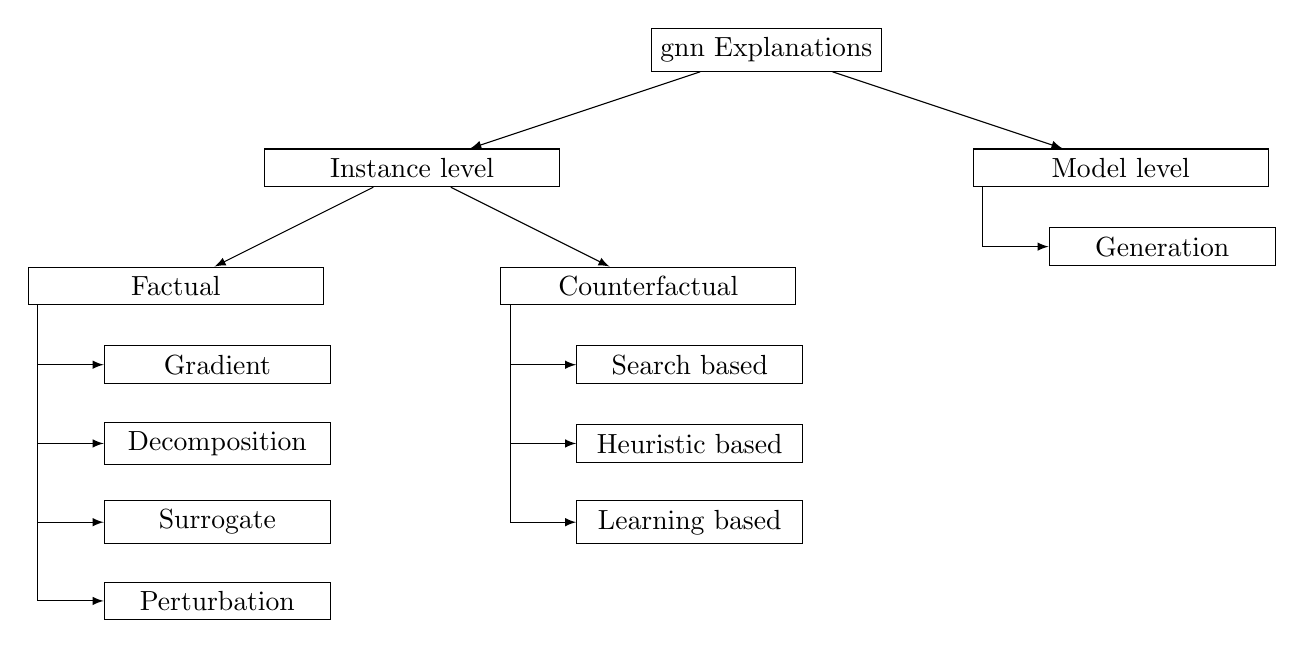
\begin{tikzpicture}[level 1/.style={sibling distance=90mm}, edge from parent/.style={->,draw}, >=latex]
    \node[root] {\gls{gnn} Explanations}
        child {node[level 2] (c1) {Instance level}
            child {node[level 3] (c3) {Factual}}
            child {node[level 3] (c4) {Counterfactual}}
        }
        child {node[level 2] (c2) {Model level}};

    \begin{scope}[every node/.style={level 4}]
        \node[below of = c3, xshift=15pt] (c31) {Gradient};
        \node[below of = c31] (c32) {Decomposition};
        \node[below of = c32] (c33) {Surrogate};
        \node[below of = c33] (c34) {Perturbation};

        \node[below of = c4, xshift=15pt] (c41) {Search based};
        \node[below of = c41] (c42) {Heuristic based};
        \node[below of = c42] (c43) {Learning based};

        \node[below of = c2, xshift=15pt] (c21) {Generation};
    \end{scope}

    \foreach \value in {1,...,4}
        \draw[->] (c3.188) |- (c3\value.west);
    \foreach \value in {1,2,3}
        \draw[->] (c4.188) |- (c4\value.west);
    \foreach \value in {1}
        \draw[->] (c2.188) |- (c2\value.west);
\end{tikzpicture}